
%(BEGIN_QUESTION)
% Copyright 2009, Tony R. Kuphaldt, released under the Creative Commons Attribution License (v 1.0)
% This means you may do almost anything with this work of mine, so long as you give me proper credit

This set of high- and low-select relays outputs a single temperature measurement signal from three transmitter inputs:

$$\includegraphics[width=15.5cm]{i03850x01.eps}$$

Calculate the output of this system given the temperature measurements shown in the diagram.  Also, calculate the output value if the lower relay (TY-25c) fails with an output equivalent to 500 $^{o}$F.

\underbar{file i03850}
%(END_QUESTION)





%(BEGIN_ANSWER)

Normal output = 1062 $^{o}$F

\vskip 10pt

Output with failed TY-25c = 500 $^{o}$F

%(END_ANSWER)





%(BEGIN_NOTES)


%INDEX% Relay, computational: selector functions

%(END_NOTES)


